% Final-presentation PDF companion to final.qmd; topic materials are preserved.
\documentclass[aspectratio=169,11pt]{beamer}
\geometry{paperwidth=20cm,paperheight=11.25cm}
\usepackage[T1]{fontenc}
\usepackage[utf8]{inputenc}
\usepackage[english]{babel}
\usepackage{amsmath,amssymb,booktabs,array,lmodern,tikz,listings}
\usetikzlibrary{arrows.meta,positioning}
\renewcommand{\familydefault}{\sfdefault}
\usefonttheme{professionalfonts}
\usetheme{default}
\definecolor{ink}{HTML}{161B24}
\definecolor{blue}{HTML}{223F91}
\definecolor{muted}{HTML}{566171}
\definecolor{orange}{HTML}{D45D00}
\definecolor{turquoise}{HTML}{008A92}
\definecolor{pale}{HTML}{F5F7FC}
\definecolor{line}{HTML}{CCD4E2}
\definecolor{paleteal}{HTML}{F0F8F8}
\definecolor{paleorange}{HTML}{FFF7EF}
\setbeamercolor{normal text}{fg=ink,bg=white}
\setbeamercolor{structure}{fg=blue}
\setbeamercolor{alerted text}{fg=orange}
\setbeamercolor{frametitle}{fg=ink,bg=white}
\setbeamercolor{block title}{fg=blue,bg=pale}
\setbeamercolor{block body}{fg=ink,bg=pale}
\setbeamerfont{frametitle}{size=\large,series=\bfseries}
\setbeamerfont{block title}{size=\normalsize,series=\bfseries}
\setbeamersize{text margin left=9mm,text margin right=9mm}
\setbeamertemplate{navigation symbols}{}
\setbeamertemplate{itemize items}[circle]
\setbeamertemplate{frametitle}{\vspace{2mm}\insertframetitle\par\vspace{2mm}{\color{line}\hrule}\vspace{2mm}}
\setbeamertemplate{footline}{\leavevmode\hbox{\begin{beamercolorbox}[wd=\paperwidth,ht=3ex,dp=1.1ex,leftskip=9mm,rightskip=9mm]{normal text}\scriptsize\color{muted}Gabriel Saco\hfill Economic freedom and firm entry--exit decisions\hfill\insertframenumber/\inserttotalframenumber\end{beamercolorbox}}}
\newcommand{\kwOrange}[1]{{\color{orange}#1}}
\newcommand{\kwTurq}[1]{{\color{turquoise}#1}}
\newcommand{\labeltext}[1]{\par{\small\bfseries\color{blue}#1\par}\vspace{1.5mm}}
\newcommand{\takeaway}[1]{\par\vspace{2.5mm}\begingroup\setlength{\fboxsep}{2.5mm}\colorbox{pale}{\begin{minipage}{\dimexpr\linewidth-5mm\relax}\small\raggedright #1\end{minipage}}\endgroup\par}
\newcommand{\panel}[3]{\begingroup\setlength{\fboxsep}{2.5mm}\colorbox{#1}{\begin{minipage}[t]{\dimexpr#2-5mm\relax}\raggedright #3\end{minipage}}\endgroup}
\setlength{\abovedisplayskip}{5pt}
\setlength{\belowdisplayskip}{5pt}
\title{Economic freedom and firm entry--exit decisions}
\author{Gabriel Saco}
\date{November 11, 2026}
\hypersetup{pdftitle={Economic freedom and firm entry-exit decisions},pdfauthor={Gabriel Saco},colorlinks=true,urlcolor=blue}


\lstset{basicstyle=\ttfamily\scriptsize,breaklines=true,columns=fullflexible,keepspaces=true,showstringspaces=false,backgroundcolor=\color{pale},frame=single,rulecolor=\color{line},
 literate={ℝ}{{$\mathbb R$}}1 {ℕ}{{$\mathbb N$}}1
 {∀}{{$\forall$}}1 {∃}{{$\exists$}}1 {→}{{$\to$}}1 {↔}{{$\leftrightarrow$}}1
 {∧}{{$\land$}}1 {∨}{{$\lor$}}1 {≤}{{$\le$}}1 {≥}{{$\ge$}}1
 {≠}{{$\ne$}}1 {∈}{{$\in$}}1 {¬}{{$\neg$}}1
 {·}{{$\cdot$}}1 {⟨}{{$\langle$}}1 {⟩}{{$\rangle$}}1
 {β}{{$\beta$}}1 {κ}{{$\kappa$}}1 {π}{{$\pi$}}1 {₀}{{$_0$}}1}
\newcommand{\sectiontag}[1]{{\scriptsize\color{muted}#1\par}\vspace{2mm}}

\begin{document}

\begin{frame}[plain]
 \begin{columns}[T,onlytextwidth]
 \begin{column}{0.78\textwidth}
 {\small\bfseries\color{blue}Universidad del Pac\'ifico}\par\vspace{2mm}
 {\small AI and Economic Modeling\par Final presentation \textperiodcentered{} Track B}
 \end{column}
 \begin{column}{0.18\textwidth}
 
\includegraphics[width=\linewidth]{reveal/logo-up.jpeg}
 \end{column}
 \end{columns}
 \vspace{9mm}
 {\LARGE\bfseries Economic freedom and\par\vspace{1mm}\color{blue}firm entry--exit decisions\par}
 \vspace{8mm}
 {\large Gabriel Saco}\par\vspace{2mm}
 Professor: Alexander Quispe\par
 \vspace{7mm}
 {\small\href{https://github.com/gsaco/ai-project}{github.com/gsaco/ai-project}\hfill\color{muted}Lima \textperiodcentered\ November 11, 2026}
\end{frame}

\begin{frame}{Why might \kwOrange{losses} exceed \kwTurq{gains}?}
 \centering
 {\small\makebox[0.48\textwidth]{Symmetry imposed}\makebox[0.48\textwidth]{Asymmetry allowed}}\par
 \vspace{1mm}
 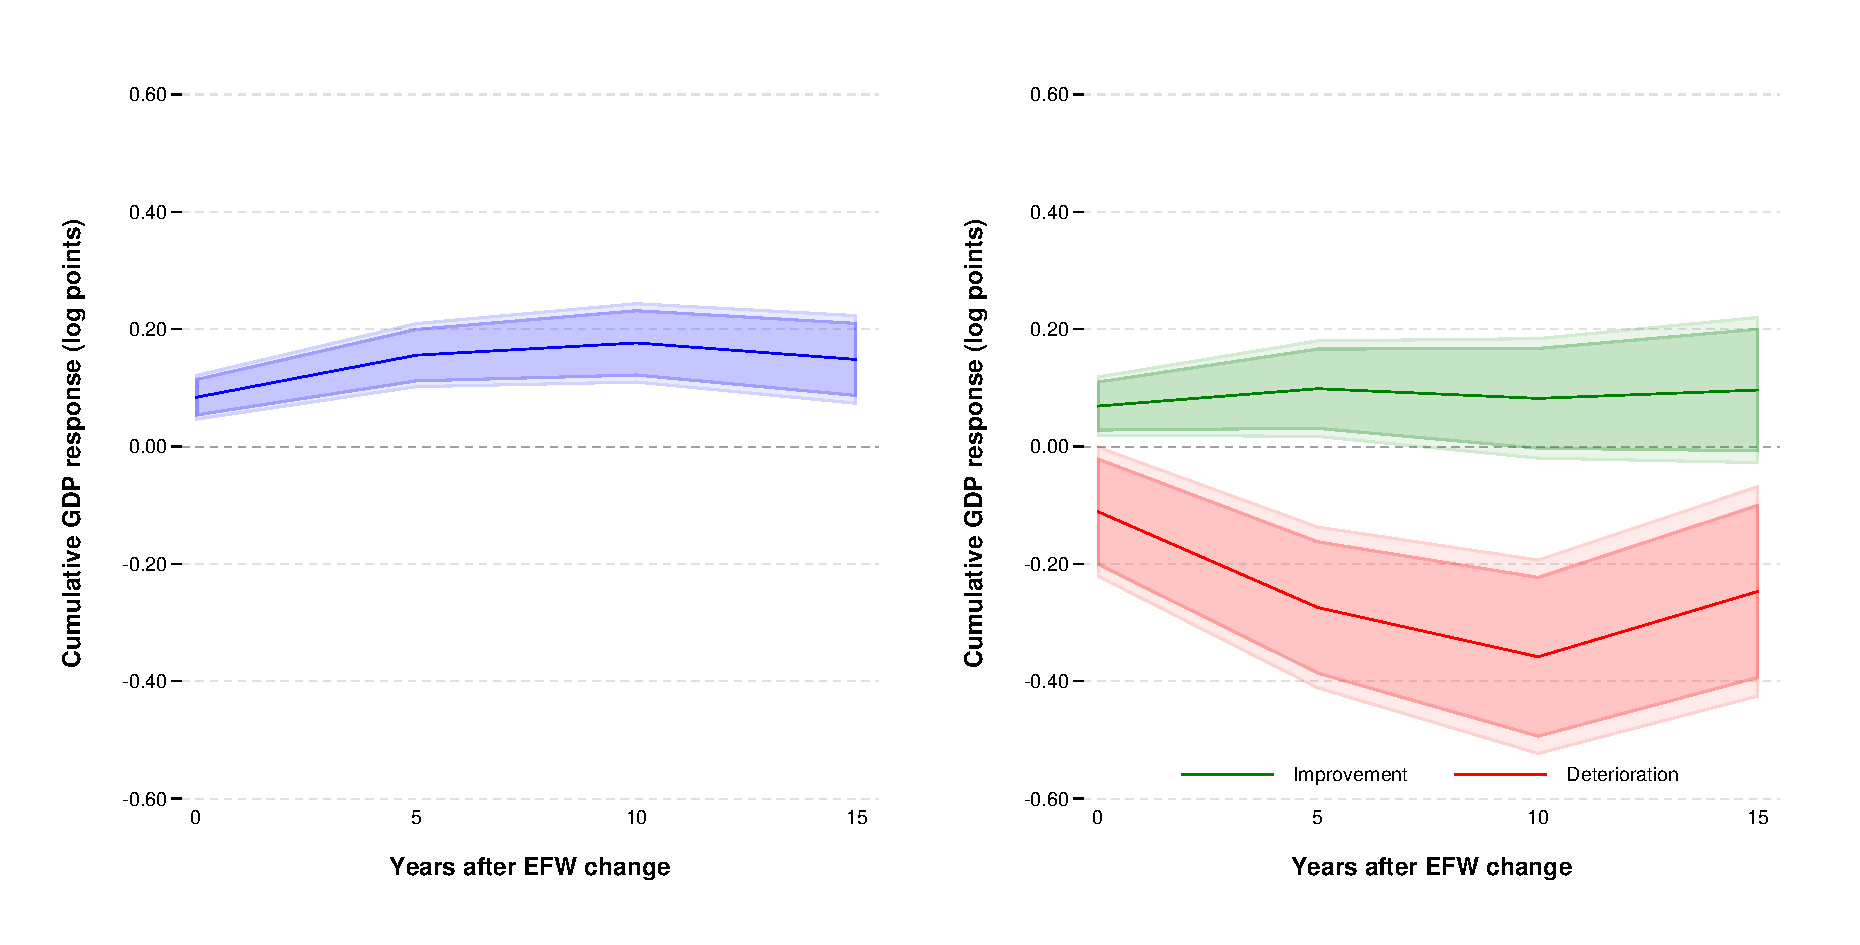
\includegraphics[width=\textwidth,height=7.4cm,keepaspectratio]{../figures/paper_main_figure.pdf}
\end{frame}

\begin{frame}{The question and the \kwOrange{conditional result}}

\sectiontag{1 \textperiodcentered{} Question and result}
\labeltext{Can equal institutional changes have unequal output effects?}
\vspace{3mm}
\panel{paleteal}{\textwidth}{\large If a temporary deterioration makes the value of continuing negative and restarting costs more than the restored business is worth, its output loss exceeds the gain from an equal improvement and persists after institutions recover.}
\vspace{6mm}
\begin{columns}[T,onlytextwidth]
\begin{column}{.47\textwidth}\labeltext{\kwOrange{Impact asymmetry}}Closure creates a discrete output loss.\end{column}
\begin{column}{.47\textwidth}\labeltext{\kwTurq{Persistence}}Costly rebuilding prevents recovery.\end{column}
\end{columns}
\takeaway{A conditional firm-level mechanism. It does not identify the thesis's aggregate coefficients.}

\end{frame}

\begin{frame}{From economic freedom to \kwTurq{two firm-level channels}}
 \small Economic freedom concerns the ability to use property, make contracts,
 and exchange. The Economic Freedom of the World (EFW) index measures several
 institutional dimensions.\par
 \vspace{2.5mm}
 {\footnotesize\centering
 \renewcommand{\arraystretch}{1.25}
 \begin{tabular}{@{}*{5}{>{\centering\arraybackslash}p{0.174\textwidth}}@{}}
 \toprule
 Area 1 & Area 2 & Area 3 & Area 4 & Area 5\\\midrule
 Size of government & Legal system and property rights & Sound money & Freedom to trade internationally & Regulation\\\bottomrule
 \end{tabular}\par}
 \vspace{3mm}
 \begin{columns}[T,onlytextwidth]
 \begin{column}{0.48\textwidth}
 \labeltext{\kwTurq{$s$: Institutionally usable property}}
 Share of existing property available for productive use under prevailing
 institutional conditions. Title disputes or restrictions on property use
 can make premises unavailable.
 \par\vspace{2mm}\kwOrange{Less usable property: $s\downarrow$}
 \end{column}
 \begin{column}{0.48\textwidth}
 \labeltext{\kwOrange{$c$: Institutional operating overhead}}
 Recurring institutional expenses paid while operating, independently of
 current output: permit renewals and fixed costs of reporting or customs
 administration.
 \par\vspace{2mm}\kwOrange{Higher operating overhead: $c\uparrow$}
 \end{column}
 \end{columns}
 \vspace{3mm}
 {\scriptsize\color{muted}\href{https://efotw.org/economic-freedom/approach}{EFW's five areas: Fraser Institute}}
\end{frame}

\begin{frame}{From \kwTurq{usable property} to production}
 \begin{columns}[T,onlytextwidth]
 \begin{column}{0.30\textwidth}\panel{pale}{\linewidth}{\centering\labeltext{Fixed property}\[\bar k>0\]\small The firm's existing stock.}\end{column}
 \begin{column}{0.03\textwidth}\vspace{8mm}$\times$\end{column}
 \begin{column}{0.30\textwidth}\panel{pale}{\linewidth}{\centering\labeltext{Usable share}\[s\in(0,1]\]\small Available under institutions.}\end{column}
 \begin{column}{0.03\textwidth}\vspace{8mm}$=$\end{column}
 \begin{column}{0.30\textwidth}\panel{paleteal}{\linewidth}{\centering\labeltext{\kwTurq{Usable property}}\[s\bar k\]\small Available for production.}\end{column}
 \end{columns}
 \vspace{4mm}
 \begin{columns}[T,onlytextwidth]
 \begin{column}{0.48\textwidth}
 \labeltext{1: Combine property with input}
 \small Assume Cobb--Douglas production:
 \[q=A(s\bar k)^{1-\alpha}x^\alpha.\]
 $x\geq0$: variable input.\par
 $A>0$: productivity.\par
 $0<\alpha<1$: output elasticity of $x$.\par
 \vspace{1mm}Output price is one: output equals revenue.
 \end{column}
 \begin{column}{0.48\textwidth}
 \labeltext{2: Choose convenient units}
 \small Measure property in units of the firm's fixed stock: $\bar k=1$.
 \[\boxed{q=As^{1-\alpha}x^\alpha.}\]
 \kwTurq{$s=0.5$:} half the existing stock is available for production.
 \end{column}
 \end{columns}
 \takeaway{An institutional shock changes the usable share $s$. The physical stock $\bar k$ stays fixed.}
\end{frame}

\begin{frame}{One experiment, \kwTurq{one changed assumption}}
 \begin{columns}[T,onlytextwidth]
 \begin{column}{0.48\textwidth}\panel{pale}{\linewidth}{\labeltext{Baseline: free restarting}\[\kappa=0\]}\end{column}
 \begin{column}{0.48\textwidth}\panel{paleteal}{\linewidth}{\labeltext{Extension: costly restarting}\[\kappa>0\]}\end{column}
 \end{columns}
 \vspace{3mm}
 {\centering\small\renewcommand{\arraystretch}{1.3}
 \begin{tabular}{@{}lcc@{}}\toprule
 Institutional path & Shock: $t=0$ & Restored: $t\geq1$\\\midrule
 Deterioration & $s_0-d$ & $s_0$\\
 No change & $s_0$ & $s_0$\\
 Improvement & $s_0+d$ & $s_0$\\\bottomrule
 \end{tabular}\par}
 \vspace{4mm}
 \begin{columns}[T,onlytextwidth]
 \begin{column}{0.48\textwidth}
 \labeltext{Same firm and known restoration}
 \small Initially open; $0<d<s_0$, $s_0+d\leq1$. Restoration is permanent and known at date~0.
 Hold $c=c_0$ and other parameters fixed.
 \end{column}
 \begin{column}{0.48\textwidth}
 \labeltext{What closure means}
 \small Free closure preserves property but dismantles the organization. No organization-preserving suspension;
 financing is available. Discount factor: $0<\beta<1$.
 \end{column}
 \end{columns}
\end{frame}

\begin{frame}{The complete \kwTurq{firm problem}}
 \begin{columns}[T,onlytextwidth]
 \begin{column}{0.48\textwidth}
 \labeltext{Activity: $a_t\in\{0,1\}$}
 \small $1$: open. $0$: closed. Initially, $a_{-1}=1$.
 \end{column}
 \begin{column}{0.48\textwidth}
 \labeltext{Variable input: $x_t\geq0$}
 \small Choose input when open; set $x_t=0$ when closed.
 \end{column}
 \end{columns}
 \vspace{3mm}
 \panel{paleteal}{\textwidth}{\labeltext{\kwTurq{Choose activity and input to maximize firm value}}
 \[\max_{\{a_t,x_t\}}\sum_{t=0}^{\infty}\beta^t
 \left[As_t^{1-\alpha}x_t^\alpha-wx_t-(F+c_0)a_t-\kappa a_t(1-a_{t-1})\right].\]}
 \vspace{4mm}
 \begin{columns}[T,onlytextwidth]
 \begin{column}{0.225\textwidth}
 \labeltext{\kwTurq{Revenue}}
 \[As_t^{1-\alpha}x_t^\alpha\]
 \small $A>0$ is productivity. Output price is one.
 \end{column}
 \begin{column}{0.205\textwidth}
 \labeltext{Input bill}
 \[wx_t\]
 \small Input quantity times its fixed unit price $w>0$.
 \end{column}
 \begin{column}{0.25\textwidth}
 \labeltext{Operating overhead}
 \[(F+c_0)a_t\]
 \small $F>0$: ordinary fixed cost.\par
 $c_0\geq0$: institutional overhead. Both paid only when open.
 \end{column}
 \begin{column}{0.255\textwidth}
 \labeltext{\kwOrange{Restart cost}}
 \[\kappa a_t(1-a_{t-1})\]
 \small Pay $\kappa\geq0$ only when closed last period and open now. Otherwise, pay zero.
 \end{column}
 \end{columns}
\end{frame}

\begin{frame}{Optimal input and \kwTurq{operating profit}}

\sectiontag{2 \textperiodcentered{} Model: solve the continuous choice first}
\begin{columns}[T,onlytextwidth]
\begin{column}{.48\textwidth}
\labeltext{1: Differentiate when operating}
\[\alpha As^{1-\alpha}x^{\alpha-1}=w.\]
\small The marginal revenue product equals the input price. Strict concavity gives the unique optimum.
\vspace{4mm}\labeltext{2: Rearrange the FOC}
\[x^*(s)=s(\alpha A/w)^{1/(1-\alpha)}.\]
\end{column}
\begin{column}{.48\textwidth}
\labeltext{3: Substitute and use $wx^*=\alpha q$}
\[q(s)=sA(\alpha A/w)^{\alpha/(1-\alpha)},\]
\[\boxed{\pi(s,c_0)=(1-\alpha)q(s)-F-c_0.}\]
\small Actual output is $y_t=a_tq(s_t)$.\par\vspace{3mm}
Define $q_0=q(s_0)$, $\pi_0=\pi(s_0,c_0)$, and $\pi_\pm=\pi(s_0\pm d,c_0)$.
\end{column}
\end{columns}
\takeaway{The input FOC is unchanged by $\kappa$: the restart bill is independent of input, and input does not change tomorrow's state.}

\end{frame}

\begin{frame}{Proposition: a temporary setback, a \kwOrange{lasting loss}}

\sectiontag{3 \textperiodcentered{} Proposition 1 in the working paper}
\small Maintain the model and matched paths: $A,w,F>0$, $c_0\geq0$, $0<\alpha,\beta<1$; initially open, $0<d<s_0$, $s_0+d\leq1$, and known permanent restoration at date one. Financing is available; closure is free, destroys the organization, and has no salvage or suspension option. No entry or reallocation.
\vspace{4mm}
\begin{columns}[T,onlytextwidth]
\begin{column}{.31\textwidth}\panel{pale}{\linewidth}{\labeltext{Normal viability}\[\pi_0>0\]\small Normal operation pays.}\end{column}
\begin{column}{.32\textwidth}\panel{pale}{\linewidth}{\labeltext{Continuation loses value}\[\pi_-+\beta V<0\]\small Future profits cannot offset the current loss.}\end{column}
\begin{column}{.33\textwidth}\panel{paleorange}{\linewidth}{\labeltext{\kwOrange{Restart is unprofitable}}\[\kappa>V\]\small Rebuilding exceeds the restored value.}\end{column}
\end{columns}
\vspace{3mm}\[V=\frac{\pi_0}{1-\beta}>0.\]
\takeaway{Unique optimal paths: $a_t^-=0$ and $a_t^0=a_t^+=1$ for every $t\geq0$.}

\end{frame}

\begin{frame}{What changes: \kwOrange{persistence}, not impact closure}

\sectiontag{3 \textperiodcentered{} Output comparison and the free-restart baseline}
\[L_t=y_t^0-y_t^-,\qquad G_t=y_t^+-y_t^0.\]
\vspace{3mm}\centering\renewcommand{\arraystretch}{1.6}
\begin{tabular}{@{}lccc@{}}\toprule
 & Impact loss $L_0$ & Impact gain $G_0$ & Loss after restoration\\\midrule
Costly restart: $\kappa>V$ & $q_0$ & $(d/s_0)q_0$ & $q_0$\\
Free restart: $\kappa=0$ & $q_0$ & $(d/s_0)q_0$ & $0$\\\bottomrule
\end{tabular}\par\vspace{4mm}\raggedright
In both cases $L_0>G_0$ because $d<s_0$. After restoration, $G_t=0$ in both cases.
\takeaway{The same adverse firm closes on impact in both experiments. Free restarting permits recovery at date one.}

\end{frame}

\begin{frame}{Proof roadmap: \kwTurq{three decisions, one comparison}}

\sectiontag{4 \textperiodcentered{} Proof progress}
\begin{enumerate}
\item \textbf{Input:} strict concavity gives $x^*(s)$, $q(s)$, and $\pi(s,c_0)$.
\vspace{3mm}\item \textbf{After restoration:} solve the active and inactive firm's values, including every possible restart date.
\vspace{3mm}\item \textbf{At date zero:} compare continuing with closing while retaining the option to reopen.
\vspace{3mm}\item \textbf{Output:} apply the chosen activity paths to the linear operating-output function $q(s)$.
\end{enumerate}
\takeaway{The delicate step is the value of closing. Zero is always feasible; it is not always the best value.}

\end{frame}

\begin{frame}{Waiting cannot improve the \kwTurq{restart value}}

\sectiontag{4 \textperiodcentered{} Lemma 2: all restart dates, including never}
\begin{columns}[T,onlytextwidth]
\begin{column}{.47\textwidth}
\labeltext{1: Active at a restored date}
\[V=\pi_0+\beta\pi_0+\cdots=\frac{\pi_0}{1-\beta}.\]
\small Closing would forgo positive profits and could add another restart bill.
\vspace{4mm}\labeltext{2: Closed at a restored date}
\small Restart after $n\geq0$ periods, then stay open:
\[\beta^n(V-\kappa).\]
Never restart: value zero.
\end{column}
\begin{column}{.49\textwidth}
\labeltext{3: Compare every delay}
\small $V>\kappa$: discounting reduces a positive payoff; restart immediately.\par\vspace{3mm}
$V<\kappa$: every finite delay has a negative payoff; never restart.\par\vspace{3mm}
$V=\kappa$: all restart dates and never restarting tie.
\vspace{3mm}\[\boxed{W=\max\{V-\kappa,0\}.}\]
\end{column}
\end{columns}
\takeaway{Once restarted, further closures cannot help because $\pi_0>0$ and $\kappa\geq0$. This covers repeated switching too.}

\end{frame}

\begin{frame}{Closure retains an \kwTurq{option to reopen}}

\sectiontag{4 \textperiodcentered{} Compare values at the same date}
\begin{columns}[T,onlytextwidth]
\begin{column}{.48\textwidth}\panel{paleteal}{\linewidth}{\labeltext{Keep operating at date zero}\[\pi_j+\beta V\]\small Current profit plus restored business value.}\end{column}
\begin{column}{.48\textwidth}\panel{paleorange}{\linewidth}{\labeltext{Close at date zero}\[\beta\max\{V-\kappa,0\}\]\small Zero current payoff plus the option to restart.}\end{column}
\end{columns}
\vspace{5mm}
\labeltext{Under the proposition's strict conditions}
\small $\kappa>V$ makes closing worth zero. Adverse continuation is negative, so closure is optimal. Normal continuation is $V>0$; favorable continuation is even larger.\par\vspace{3mm}
With $\kappa=0$, closure is worth $\beta V$. Since $\pi_-<0$, the adverse firm still closes, but reopens at date one.
\takeaway{$a_t$ is binary: its optimality condition is a value comparison, not a derivative with respect to activity.}

\end{frame}

\begin{frame}{The conditions \kwTurq{can hold together}}

\sectiontag{4 \textperiodcentered{} Nonempty parameter region}
\small $A=2$, $\alpha=0.5$, $w=1.25$, $F=0.30$, $c_0=0.09$, $s_0=0.50$, $d=0.20$, $\beta=0.90$, $\kappa=0.40$.
\vspace{4mm}
\begin{columns}[T,onlytextwidth]
\begin{column}{.47\textwidth}\labeltext{Compute from the primitives}
\[q_0=0.80,\quad \pi_0=0.01,\quad V=0.10,\]
\[\pi_-=-0.15,\qquad \pi_+=0.17.\]
\labeltext{Check the strict inequalities}
\[\pi_-+\beta V=-0.06<0,\qquad \kappa>V.\]
\end{column}
\begin{column}{.49\textwidth}\labeltext{Why a thin margin matters}
\small Permanent closure requires
\[\frac{\pi_0}{(1-\alpha)q_0}<(1-\beta)\frac d{s_0}.\]
Here $0.025<0.04$. Normal operation is profitable, but future earnings are small relative to the shock loss.
\end{column}
\end{columns}
\takeaway{All inequalities are strict: a neighborhood of this example also satisfies the proposition. The result is not universal.}

\end{frame}

\begin{frame}{Proof status: \kwTurq{done}, difficult, open}

\sectiontag{4 \textperiodcentered{} Analytic proofs versus remaining research}
\begin{columns}[T,onlytextwidth]
\begin{column}{.31\textwidth}\labeltext{\kwTurq{Proved in the paper}}
\small Unique input optimum.\par\vspace{2mm}All delayed restart values.\par\vspace{2mm}Strict persistence and the complete closure threshold.\par\vspace{2mm}Cheap-suspension threshold.
\end{column}
\begin{column}{.31\textwidth}\labeltext{The difficult step}
\small Accounting for closure's option value.\par\vspace{2mm}Ruling out arbitrary delay and repeated switching.\par\vspace{2mm}Separating impact from recovery.
\end{column}
\begin{column}{.32\textwidth}\labeltext{\kwOrange{Still open}}
\small Entry and reallocation.\par\vspace{2mm}A heterogeneous-firm equilibrium.\par\vspace{2mm}Empirical measurement of restart and preservation costs.\par\vspace{2mm}Independent assessment of the remaining AI contributions.
\end{column}
\end{columns}
\takeaway{Analytic completion, numerical checks, Lean coverage, and independent author review are separate claims.}

\end{frame}

\begin{frame}{Three reproduced cases: \kwTurq{same model}}

\sectiontag{5 \textperiodcentered{} Numerical illustrations, not calibration}
\centering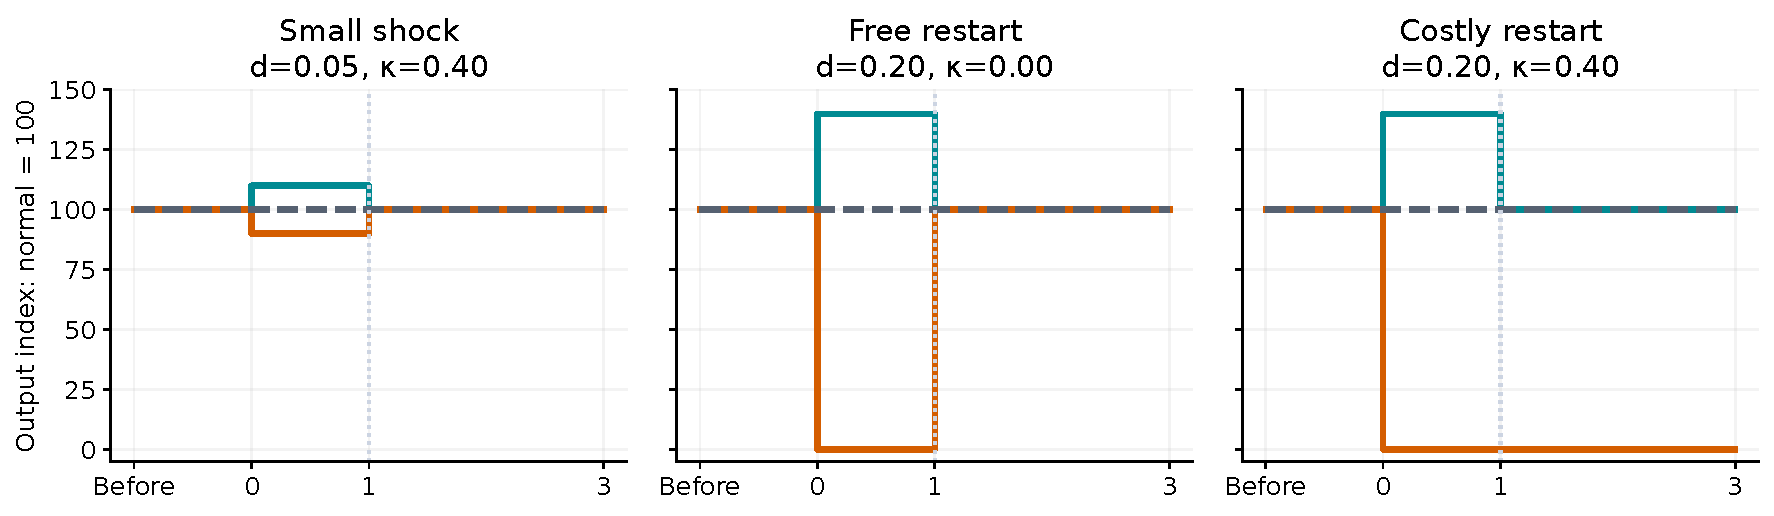
\includegraphics[width=\textwidth,height=5.5cm,keepaspectratio]{final-assets/cases.pdf}\par
\small\kwTurq{Improvement}\quad\kwOrange{Deterioration}\quad\textcolor{muted}{No change (dashed)}\par\vspace{4mm}\raggedright
\takeaway{Small shocks: keep operating. Large shocks: close. Restart costs distinguish recovery from permanent inactivity.}

\end{frame}

\begin{frame}{Where does each \kwOrange{operating regime} occur?}

\sectiontag{5 \textperiodcentered{} Proposition 2 and parameter comparisons}
\small Strict closure if
\[(1-\alpha)q_0\frac d{s_0}>\pi_0+\beta\min\{\kappa,V\}.\]
\centering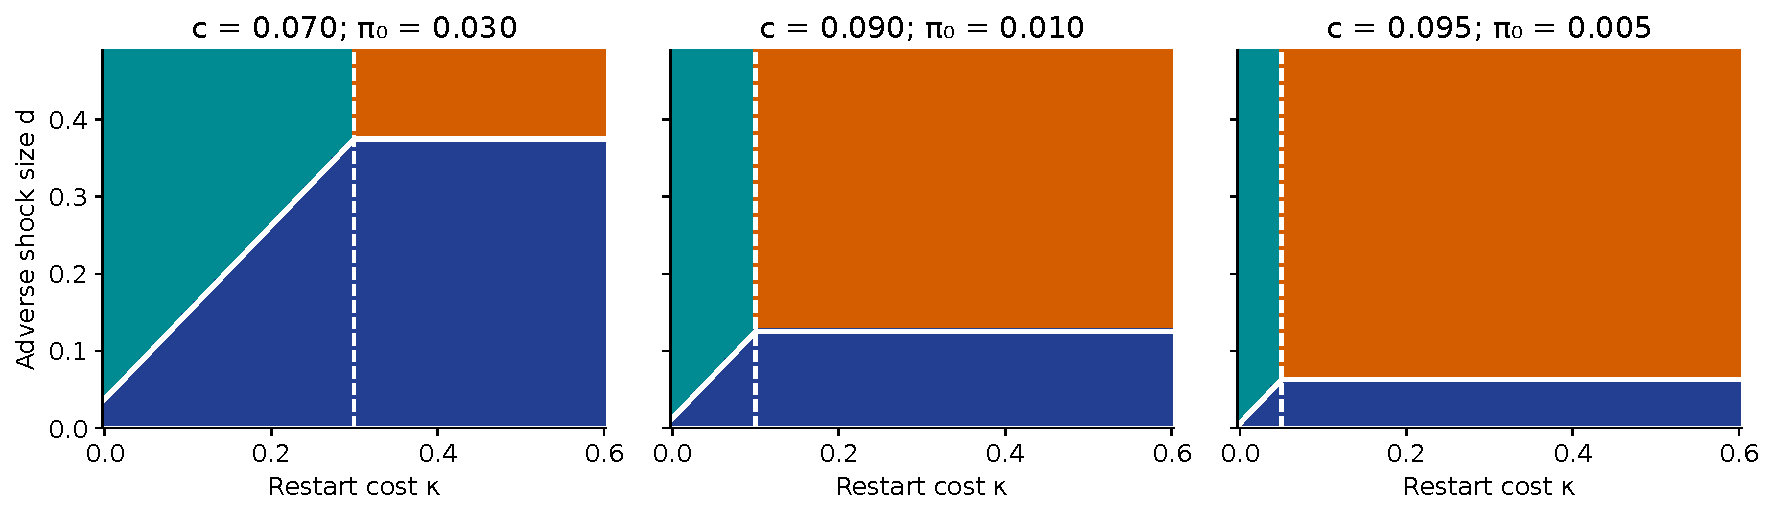
\includegraphics[width=\textwidth,height=4.4cm,keepaspectratio]{final-assets/regimes.pdf}\par
\small\textcolor{blue}{Keep operating}\quad\kwTurq{Close and reopen}\quad\kwOrange{Close permanently}\par\vspace{2mm}\raggedright
\takeaway{Higher $\kappa$ can discourage closure today; higher $c_0$ lowers normal margins and expands the permanent-closure region. White curves mark closure indifference; dashed lines mark $\kappa=V$.}

\end{frame}

\begin{frame}{Explore the \kwTurq{decision margins}}

\sectiontag{5 \textperiodcentered{} Interactive companion: shock, restart cost, and overhead}
\renewcommand{\arraystretch}{1.4}\centering
\begin{tabular}{@{}lrrrl@{}}\toprule
Experiment & $d$ & $\kappa$ & $c_0$ & Adverse-firm path\\\midrule
Small shock & .05 & .40 & .09 & Keep operating\\
Free restart & .20 & 0 & .09 & Close, then reopen\\
Costly restart & .20 & .40 & .09 & Close permanently\\
Stronger normal margin & .20 & .40 & .07 & Keep operating\\
Avoid a costly restart & .10 & .40 & .09 & Keep operating\\\bottomrule
\end{tabular}\par\vspace{4mm}\raggedright
\labeltext{What to vary live}
\small First compare the three topic cases. Then lower $c_0$, holding the shock fixed. Finally hold $d=0.10$ and compare $\kappa=0$ with $\kappa=0.40$.
\takeaway{The interactive version updates both values and output paths. It keeps $c_0$ constant over time within each experiment.}

\end{frame}

\begin{frame}{First robustness test: \kwTurq{cheap suspension}}

\sectiontag{5 \textperiodcentered{} Proposition 3: preserve the organization for a cost $h$}
\small At date zero, suspension produces nothing, costs $h\geq0$ in total, and preserves the organization for free resumption at date one. It replaces operating overhead for that period.
\[\text{Suspend: }-h+\beta V;\qquad\text{close: }0;\qquad\text{operate: }\pi_-+\beta V<0.\]
\centering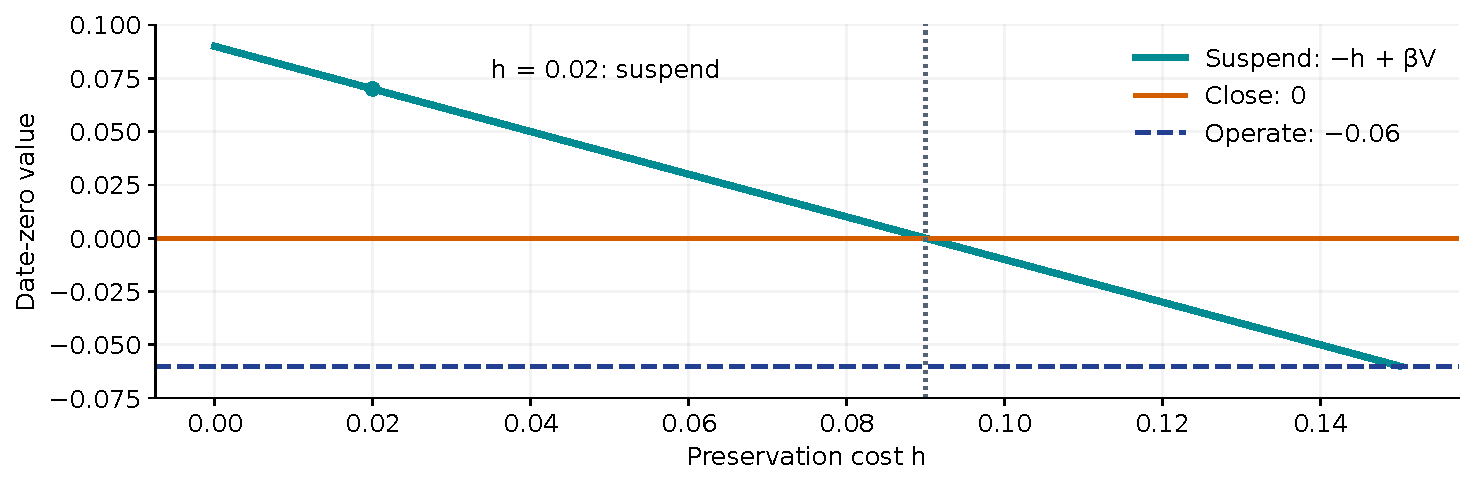
\includegraphics[width=.98\textwidth,height=4.2cm,keepaspectratio]{final-assets/suspension.pdf}\par\raggedright
\takeaway{If $h<\beta V$, suspension strictly wins. Impact loss remains, but production fully recovers at date one. At $h=\beta V$, suspension and closure tie.}

\end{frame}

\begin{frame}{What the calculations \kwTurq{check} and leave open}

\sectiontag{5 \textperiodcentered{} Scope of the numerical evidence}
\begin{columns}[T,onlytextwidth]
\begin{column}{.48\textwidth}\labeltext{Checked}
\small Symbolic FOC and numerical input optimum.\par\vspace{2mm}Three topic cases reproduced.\par\vspace{2mm}168 parameter points: compare closed-form decisions with all five-date activity sequences and an exact stationary tail.\par\vspace{2mm}151 suspension costs; delay, tie, and browser/Python checks.
\end{column}
\begin{column}{.48\textwidth}\labeltext{\kwOrange{Not established by those checks}}
\small A finite grid is not a proof over all parameters.\par\vspace{2mm}No estimated EFW shock or calibrated GDP effect.\par\vspace{2mm}Entry and heterogeneity remain open: $\kappa>V$ does not exclude favorable date-zero entry.\par\vspace{2mm}Fixed-cohort totals are accounting, not general equilibrium.
\end{column}
\end{columns}
\takeaway{Even when $\kappa>V$, an otherwise identical inactive owner can enter during the improvement if $\pi_++\beta V-\kappa>0$. Entry and reallocation can alter the aggregate comparison.}

\end{frame}

\begin{frame}[fragile]{Lean checks \kwTurq{every possible restart path}}
\sectiontag{6 \textperiodcentered{} Paper statement, Lean statement, and proof excerpt}
\begin{columns}[T,onlytextwidth]
\begin{column}{.35\textwidth}
\labeltext{Paper: Lemma 2, costly-restart clause}
\small Under A1--A6, ``permanent inactivity is uniquely optimal if $V<\kappa$.''
\[V=\frac{\pi_0}{1-\beta},\qquad \pi_0>0,\quad0<\beta<1.\]
\vspace{2mm}\labeltext{Read the formal statement}
\small \texttt{pi} is $\pi_0$; \texttt{false} means initially closed.\par\vspace{2mm}
\texttt{a} is any infinite sequence of activity choices.\par\vspace{2mm}
The maximum is zero. Only the never-restart path attains it.
\end{column}
\begin{column}{.62\textwidth}
\labeltext{Actual Lean statement}
\begin{lstlisting}[basicstyle=\ttfamily\fontsize{8.6}{10}\selectfont]
lemma restored_inactive_optimal_iff_inactive {pi beta kappa : ℝ}
    (hpi : 0 < pi) (hbeta0 : 0 < beta) (hbeta1 : beta < 1)
    (hkappa : 0 ≤ kappa) (hkgt : pi / (1 - beta) < kappa)
    (a : ActivityPath) :
    restoredPathValue pi beta kappa false a =
      max (pi / (1 - beta) - kappa) 0 ↔ a = alwaysInactive := by
\end{lstlisting}
\labeltext{Proof excerpt: equality forces the inactive path}
\begin{lstlisting}[basicstyle=\ttfamily\fontsize{8.6}{10}\selectfont]
  rw [restoredPathValue_eq_potential_iff_slack_zero
    hpi hbeta0 hbeta1 hkappa]
  constructor
  · exact tight_inactive_forces_inactive
      hpi hbeta0 hbeta1 hkappa hkgt a
\end{lstlisting}
{\scriptsize\color{muted}\texttt{lean/MainTheorems.lean}; statement line breaks adapted.}
\end{column}
\end{columns}
\takeaway{The proof bounds the infinite discounted payoff of every path. Equality requires no profitable decision to be forgone at any date; here that forces permanent inactivity.}
\end{frame}

\begin{frame}{Lean: \kwTurq{verified scope} and the remaining gap}
\sectiontag{6 \textperiodcentered{} Compiling a proof and checking its economic meaning are different tasks}
\begin{columns}[T,onlytextwidth]
\begin{column}{.47\textwidth}
\labeltext{What has compiled}
\small Six formal counterparts of the paper's numbered results, with no \texttt{sorry}.\par\vspace{4mm}
The input optimum and the reduced activity problem, including arbitrary infinite paths.\par\vspace{4mm}
Switching thresholds, suspension comparisons, and positive-total log comparisons.
\end{column}
\begin{column}{.49\textwidth}
\labeltext{\kwOrange{What remains open}}
\small The formal bridge from joint input/activity maximization to the reduced activity problem.\par\vspace{4mm}
This includes unoptimized plans whose discounted losses are infinite.\par\vspace{4mm}
The required fast check passed. Full source-correspondence certification remains incomplete.
\end{column}
\end{columns}
\vspace{4mm}
{\scriptsize\color{muted}Paper version: merged commit \texttt{a15ed978}. Complete declarations and command records accompany the paper.}
\takeaway{Lean checks the specified input and reduced dynamic problems. I do not yet claim verification of the full original optimization problem.}
\end{frame}

\begin{frame}{The AI-assisted step I \kwOrange{checked by hand}}

\sectiontag{7 \textperiodcentered{} Selected derivation: closure with an option to reopen}
\begin{enumerate}
\item At date one, immediate restarting yields $V-\kappa$.
\vspace{2mm}\item Restarting $n$ periods later yields $\beta^n(V-\kappa)$.
\vspace{2mm}\item Include never restarting, with value zero.
\vspace{2mm}\item Compare positive, zero, and negative $V-\kappa$; discount the best value once to date zero.
\end{enumerate}
\vspace{3mm}\[\boxed{\text{Closing value at date zero}=\beta\max\{V-\kappa,0\}.}\]
\takeaway{An AI-generated uniqueness helper allowed $\beta=0$: then future actions do not affect value. The paper already requires $\beta>0$. That diagnostic is separate from my handwritten closure-value check.}

\end{frame}

\begin{frame}{My handwritten check and \kwTurq{assessment}}
\sectiontag{7 \textperiodcentered{} My revision \textperiodcentered{} November 9, 2026}
\begin{columns}[T,onlytextwidth]
\begin{column}{.64\textwidth}
\begin{tikzpicture}
\path[use as bounding box] (0,0) rectangle (11.35,7.65);
\begin{pgfinterruptboundingbox}
\clip (0,0) rectangle (11.35,7.65);
\node[anchor=north west,inner sep=0pt] at (-11.888,10.099)
 {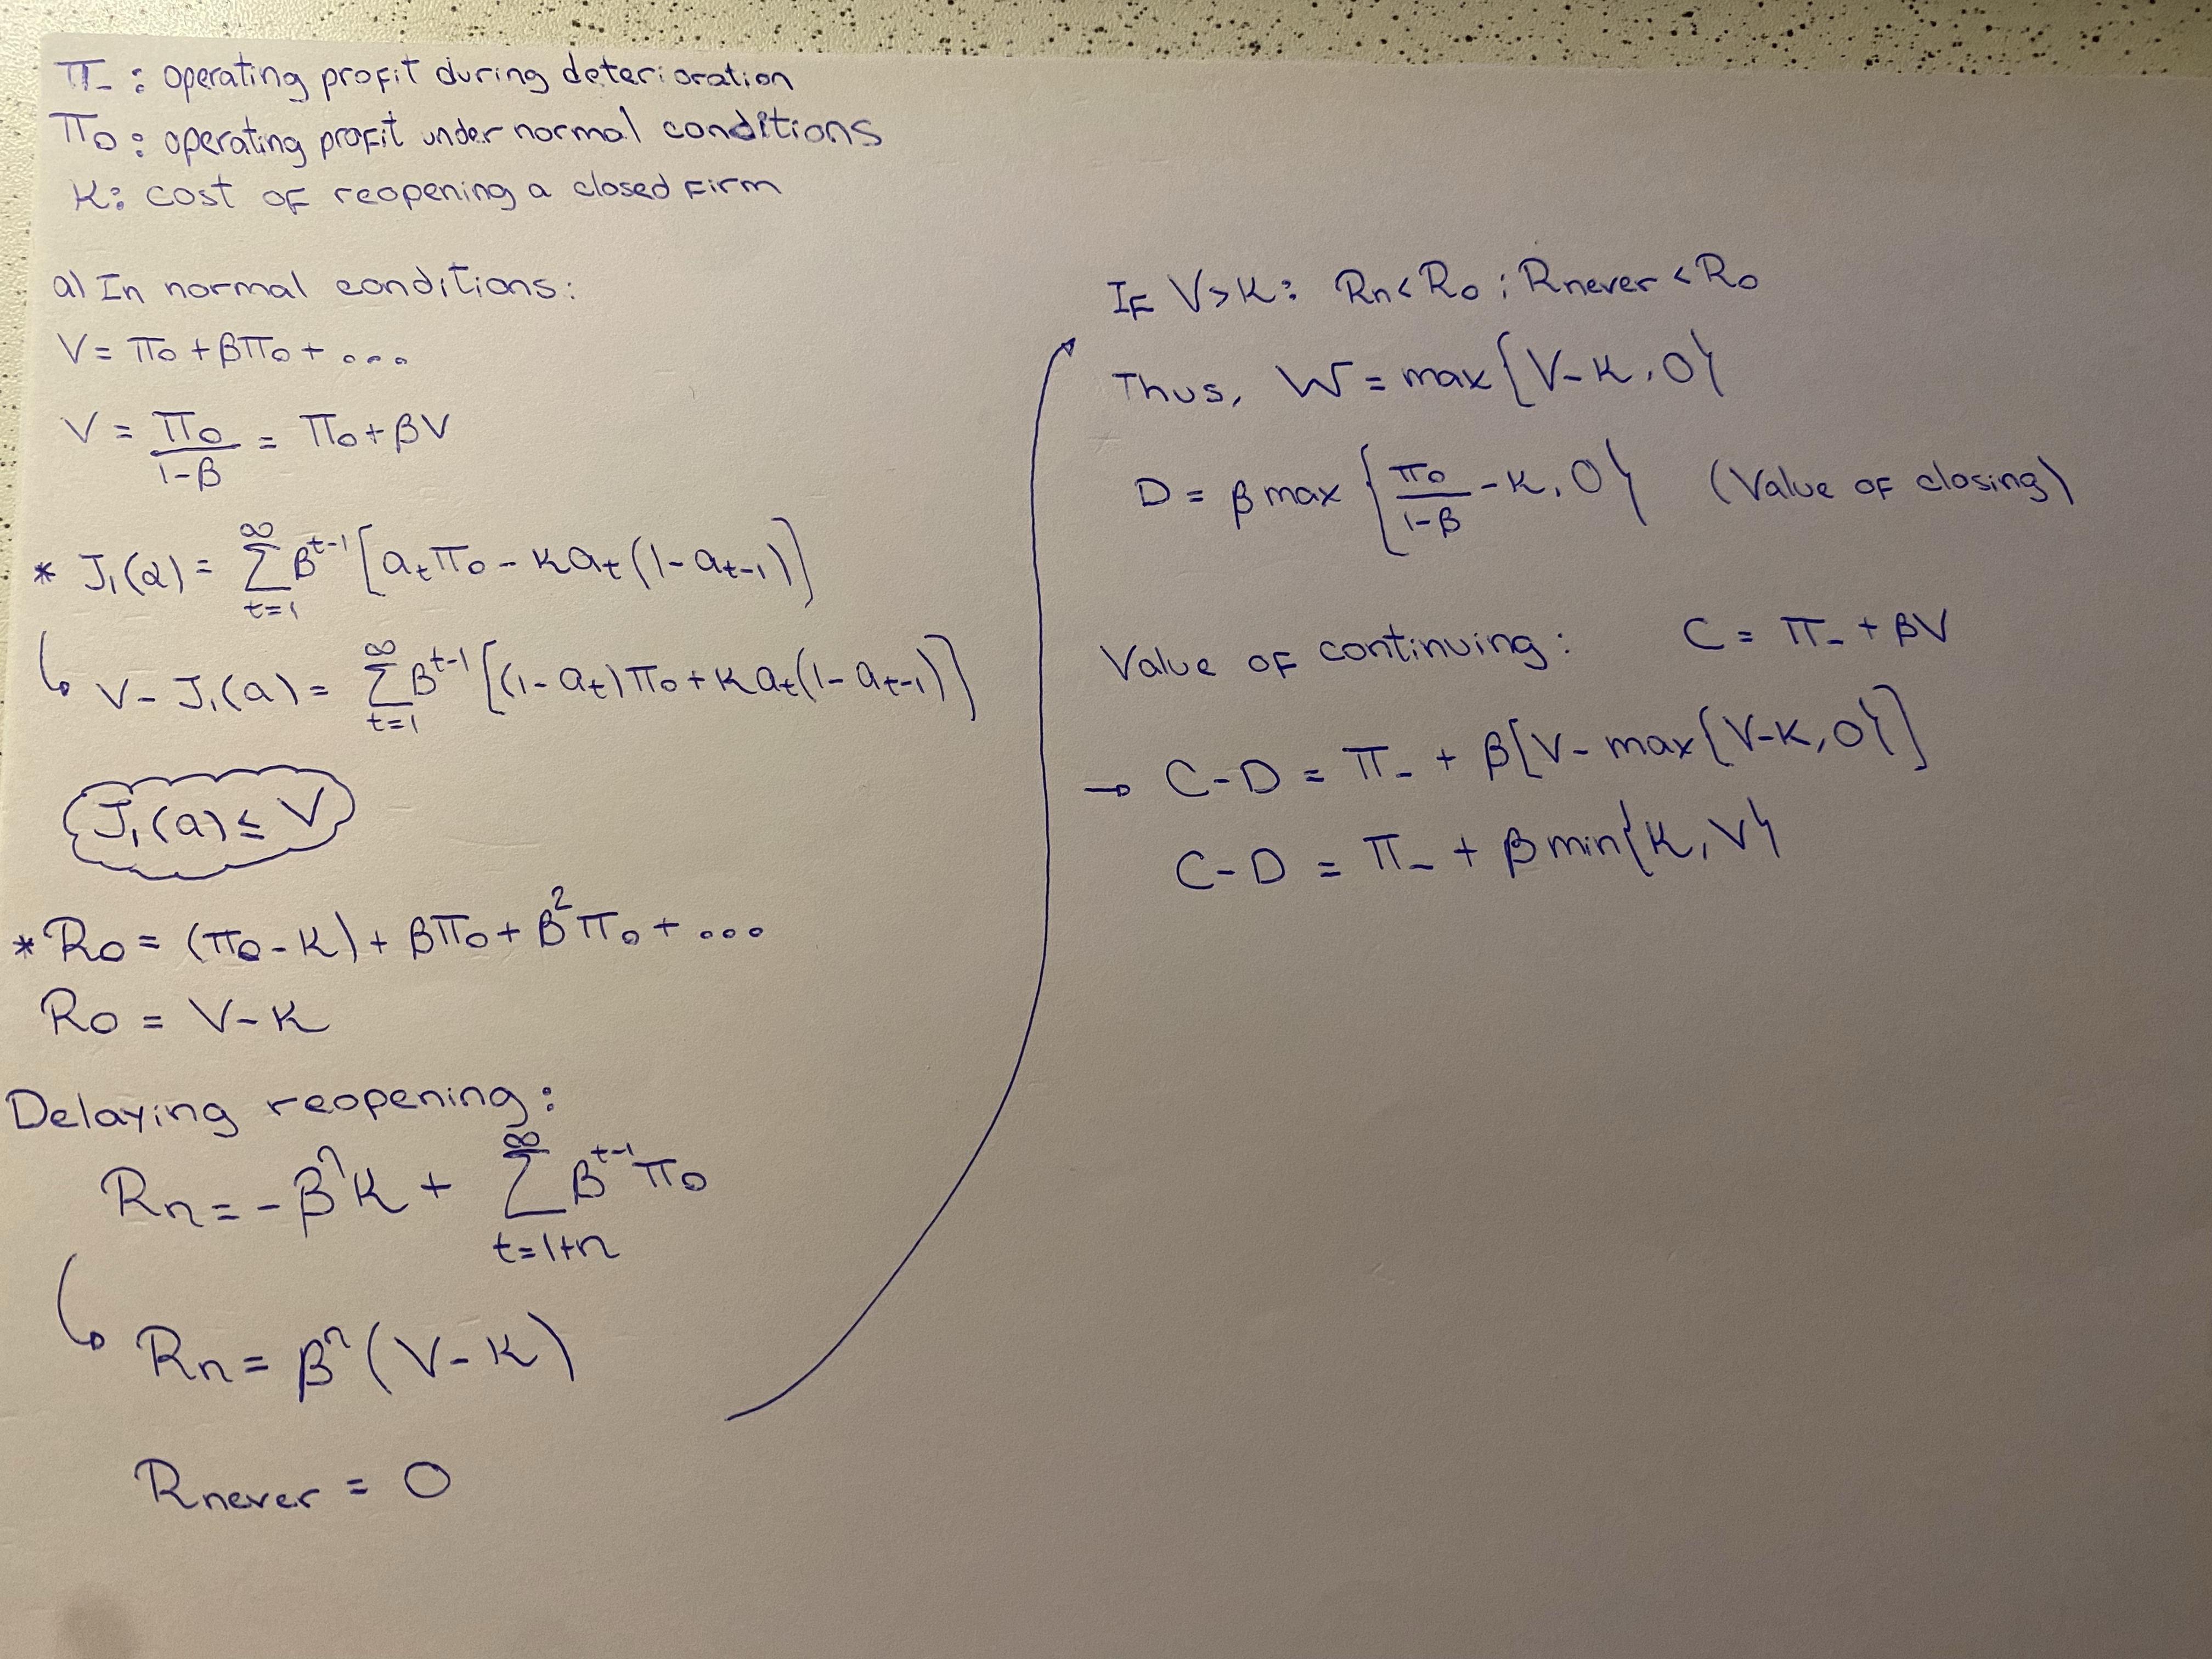
\includegraphics[width=24.086cm]{../hand/final/handwritten-revision-2026-11-09.png}};
\end{pgfinterruptboundingbox}
\end{tikzpicture}
\end{column}
\begin{column}{.32\textwidth}
\labeltext{\kwTurq{My verdict}}
{\Large ``I accept it.''}\par\vspace{7mm}
\labeltext{My restart calculation}
\[R_n=\beta^n(V-\kappa),\qquad n\geq0,\]
\[R_{\mathrm{never}}=0.\]
\small Compare delayed reopening with never reopening, then discount once to date zero.\par\vspace{6mm}
{\scriptsize\color{muted}Enlarged excerpt of my original photograph. The complete page is in backup slide 29.}
\end{column}
\end{columns}
\end{frame}

\begin{frame}{Three questions for \kwTurq{class discussion}}

\sectiontag{8 \textperiodcentered{} Discussion: 15 minutes}
\begin{enumerate}
\item \textbf{Suspension:} what observable evidence would distinguish temporary shutdown from organization-destroying closure? Which costs should $h$ include?
\vspace{6mm}\item \textbf{Aggregation:} what is the smallest model of heterogeneous firms, entry, and reallocation that could preserve the loss--gain comparison?
\vspace{6mm}\item \textbf{Timing and margins:} should the next extension vary the duration of restoration or relax perfect foresight? How would we identify the fragile firms?
\end{enumerate}

\end{frame}

\begin{frame}{Literature and \kwTurq{reproducible materials}}

\small
\textbf{Dixit (1989).} \emph{Entry and Exit Decisions under Uncertainty}. JPE 97(3), 620--638. Sunk costs and the distinction between incumbency and entry.\par\vspace{4mm}
\textbf{Dixit (1992).} \emph{Investment and Hysteresis}. JEP 6(1), 107--132. Suspension versus abandonment.\par\vspace{4mm}
\textbf{Lawson, Murphy, and Mitchell (2025).} \emph{Economic Freedom of the World}. Institutional measurement framework.\par\vspace{5mm}
\href{https://github.com/gsaco/ai-project}{github.com/gsaco/ai-project}: working paper, code and check logs, Lean artifacts, and AI record. The October topic submission is preserved.
\takeaway{I use an established sunk-cost mechanism in a deterministic institutional experiment. The contribution is the precise conditional comparison and its limits.}

\end{frame}

\begin{frame}{Backup: \kwTurq{all switching regions and ties}}

\labeltext{Continuation minus closure value}
\[\pi_-+\beta V-\beta\max\{V-\kappa,0\}
=\pi_0-(1-\alpha)q_0\frac d{s_0}+\beta\min\{\kappa,V\}.\]
\small A negative difference implies closure; a positive one implies operation; zero gives indifference.\par\vspace{4mm}
After closure: $\kappa<V$ implies immediate restart; $\kappa>V$ implies never restarting; $\kappa=V$ allows any restart date or none.\par\vspace{4mm}
Under every optimal selection, $L_t\geq G_t\geq0$. Strictness occurs at impact exactly when the adverse firm closes; later exactly when it remains closed.
\takeaway{The numerical convention keeps operating at a closure tie and declines a zero-value restart. The strict proposition does not depend on that convention.}

\end{frame}

\begin{frame}{Backup: \kwTurq{logs require positive totals}}

\labeltext{A fixed-cohort accounting extension}
\[Y_t^j=B+Ny_t^j,\qquad B>0,\quad N>0.\]
\small Under Proposition 1, strict level asymmetry implies
\[2Y_t^0>Y_t^-+Y_t^+\geq2\sqrt{Y_t^-Y_t^+},\]
\[(Y_t^0)^2>Y_t^-Y_t^+\quad\Longrightarrow\quad
\log Y_t^0-\log Y_t^->\log Y_t^+-\log Y_t^0.\]
\vspace{4mm}\small Common population cancels from per-capita log differences. A closed firm's log output is undefined. Even symmetric level changes can be asymmetric in logs.
\takeaway{This is not a model of GDP: it holds background output and the cohort fixed and omits entry, prices, and reallocation.}

\end{frame}
\begin{frame}{Backup: my \kwTurq{original handwritten revision}}
\centering
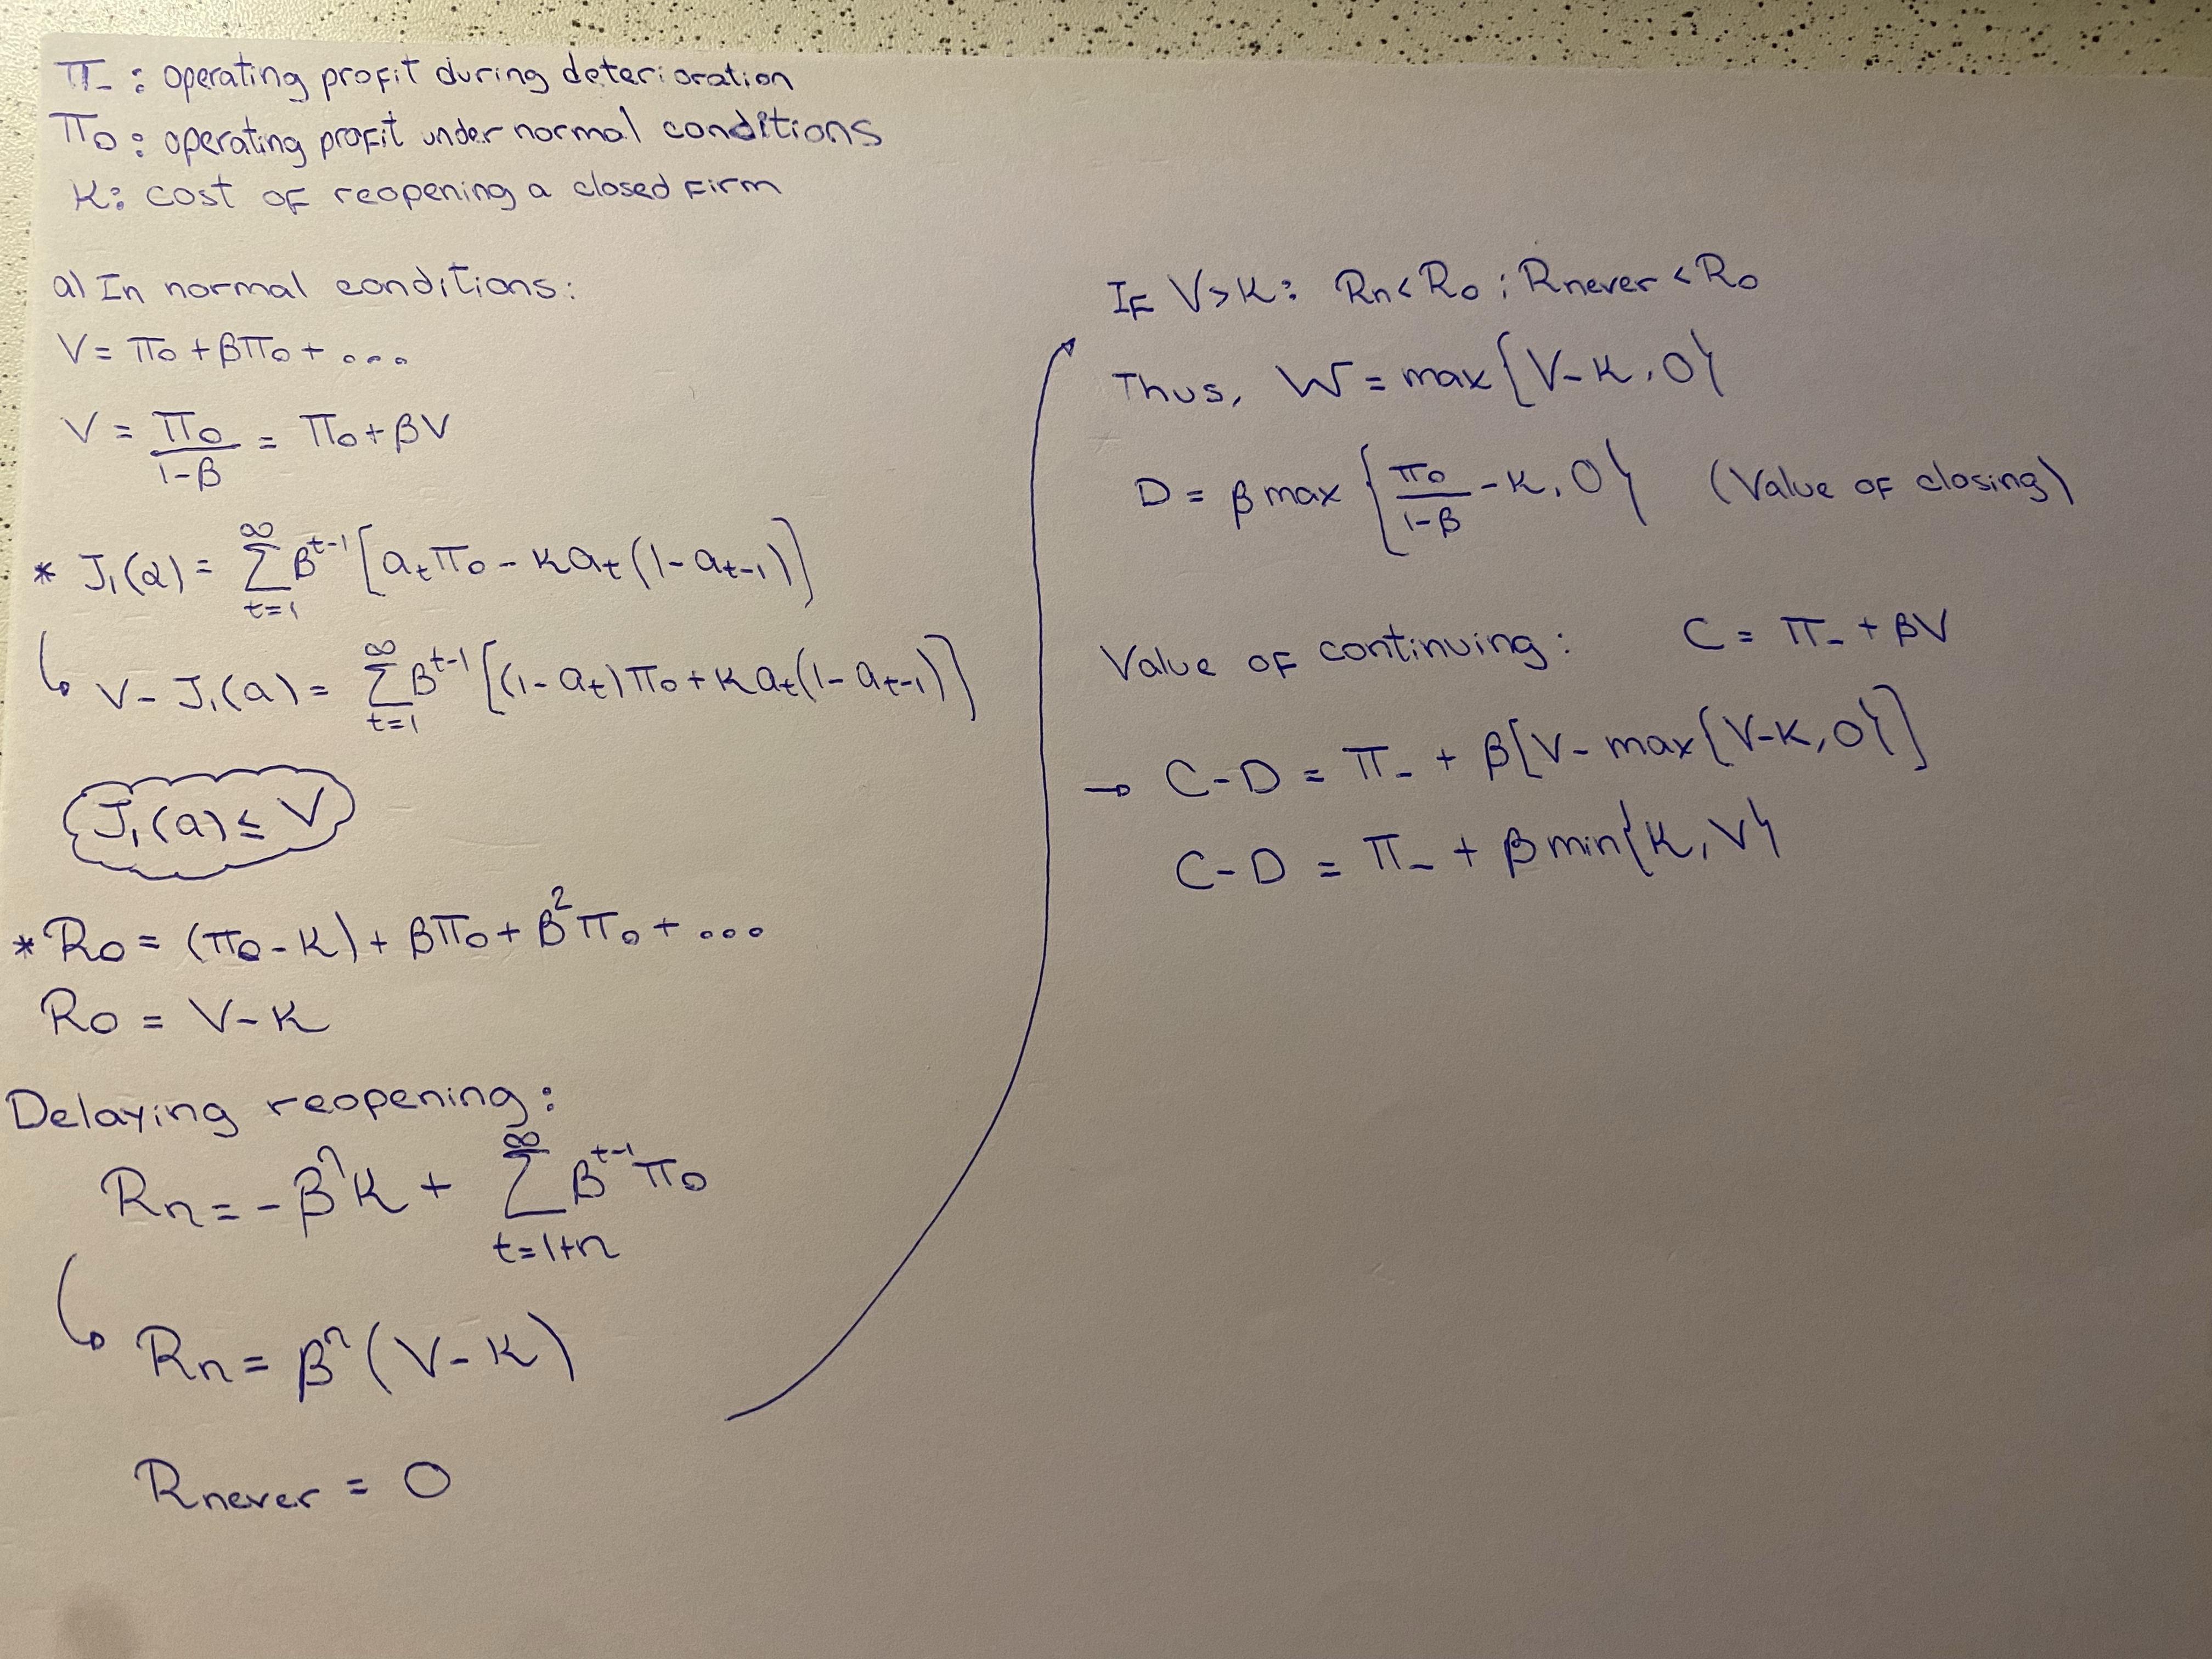
\includegraphics[width=\textwidth,height=8.45cm,keepaspectratio]{../hand/final/handwritten-revision-2026-11-09.png}
\end{frame}

\end{document}
